\documentclass[10pt]{article}

\def\Type{LessonCaelan}
\def\TypeNum{Lesson 20}
\def\TypeTitle{Intro to Probability and Discrete Random Variables\\Solutions }
\def\Semester{Fall 2021} %Not Used 
\def\Course{MATH 1190 \& 1210}

\usepackage{preambleDJ}



%%%%%%%%%%%% BEGIN DOCUMENT %%%%%%%%%%%%%%%
%%%%%%%%%%%% BEGIN DOCUMENT %%%%%%%%%%%%%%%
%%%%%%%%%%%% BEGIN DOCUMENT %%%%%%%%%%%%%%%
%%%%%%%%%%%% BEGIN DOCUMENT %%%%%%%%%%%%%%%
%%%%%%%%%%%% BEGIN DOCUMENT %%%%%%%%%%%%%%%

\begin{document}


\thispagestyle{firstpage}
\pagestyle{otherpages}
\vs{0.65}



\textbf{Intended Learning Outcomes}
After this lesson, you will be able to 

\begin{itemize}
    \item List outcomes in the sample space or an event of a random process. (\target{P1})
    \item Determine if a random variable is discrete.(\target{P1})
    \item Find a probability of an event when the sample space is finite. (\target{P1})
    %\item Use summations to find the probability that an event modeled by a discrete random variable occurs. (\target{P1})
    \item Determine and use the probability mass function and its properties of a discrete random variable. (\target{P1})
    \item Sketch the histogram representing a probability mass function. (\target{P1})
\end{itemize}

\vspace{-0.5cm}

\hrulefill

\vspace{0.2cm}

\fbox{
\begin{minipage}{0.95\textwidth}
Fill in the blanks.
\begin{itemize}
\item An \unlinebt{1.2}{experiment}{.18} is a process that can be infinitely repeated by which we observe something uncertain.

\item An \unlinebt{1.2}{outcome}{.18} is a result of one iteration of an experiment. 

\item The  \unlinebt{1.2}{sample space}{.18}  of a random process is the collection of all its possible outcomes.

\item An  \unlinebt{1.2}{event}{.18}  is a collection of outcomes from the sample space.
\end{itemize}
\end{minipage}
}

\exercise{\bf\color{Orange}P1} An opaque bag contains 1 {\color{red}red} marble, 1 {\color{ForestGreen}green} marble, and 1 {\color{blue}blue} marble. ({\it Hint:} For example, denote outcomes using notation like {\color{red}R}, {\color{ForestGreen}G}, or {\color{blue}B}, as appropriate!)
    \begin{itemize}
    \item[(a)] In an experiment where one marble is drawn randomly from the bag and the color of the marble is recorded, what is the sample space $S$?

    {\Large
    \[
    S =\unlineb{4}{\{R,B,G\}}
    \]
    }

    \item[(b)] In another experiment, one marble is drawn randomly from the bag, the color of the marble is recorded, the marble is placed back in the bag, and then a second marble is drawn, its color recorded, and then the marble is placed back in the bag. What is the sample space $S$? ({\bf Note:} we call this drawing {\bf with replacement}.)

    {\Large
    \[
    S = \unlineb{4}{\{RR,RG,RB,GR,GG,GB,BR,BG,BB\}}
    \]
    }

    \item[(c)] In another experiment, one marble is drawn randomly from the bag, the color of the marble is recorded, the marble is NOT placed back in the bag, and then a second marble is drawn, its color recorded, and then the marble is NOT placed back in the bag. What is the sample space $S$? ({\bf Note:} we call this drawing {\bf without replacement}.)

    {\Large
    \[
    S = \unlineb{4}{\{RG,RB,GR,GB,BR,BG\}}
    \]
    }
    
    \end{itemize}

%%%%%%%%%
\newpage%
%%%%%%%%%

{\bf Discrete Random Variables and Probabilities of Events}
\vs{-.15}
\important{Key Definitions}{\begin{itemize}
    \item A \unlineb{2}{\text{Random Variable}} assigns a number (not necessarily unique) to each outcome in a sample space.
    \item A \unlineb{2}{\text{Discrete Random Variable}} is a random variable that can only take on a {\em countable} number of values (e.g. $1$,$2$,$3$, $\dots$.) Frequently there will only be a {\em finite} number of these values.
\item When all outcomes in the sample space $S$ are equally likely, then the probability of an event $E$, denoted as $P(E)$, can be computed as:

\[ P(E) = \dfrac{\text{size of the event}}{\text{size of the sample space}} \]

\item For a discrete random variable $X$, the {\bf probability mass function} (PMF) $p(x)$ describes the probability of all possible outcomes, $x$, in the sample space $S$.  That is  $p(x)=P(X=x)$ for each $x \in S$
\end{itemize}
}
\example Given a six-sided die
\tasksI{2}{
\task The {\em experiment} \blue{ rolling the die. }
\task  Number of {\em Outcomes}: \blue{There are $6$ outcomes corresponding to the number on each face} \vs{.25}
\task The {\em sample space} \blue{$S=\{1,2,3,4,5,6\}$}.
\task  {\em Discrete random variable} $X$  \blue{The (random) outcome of the roll of one die.}\vs{.25}
}

\tasksA{2}{
\task What is $P(X=2)$? \blue{$P(X=2)=\dfrac{1}{6}$}
\task What is $P(X\leq 2)$? \\\blue{$\ds P(X\leq 2)=P(X=1)+P(x=2)=\frac{1}{6}+\frac{1}{6}=\frac{2}{6}=\frac{1}{3}$}
\vs{.5}
\task  Create the probability mass function, $p(x)$. \\Recall that $p(x)=P(X=x)$\\\\
{\renewcommand{\arraystretch}{2}
        \begin{tabularx}{2in}{c|cccccc} 
            \hline
           $x$  & 1 & 2 & 3 & 4&5&6 \\
           \hline
           $p(x)$  &\blue{$\dfrac{1}{6}$} &\blue{$\dfrac{1}{6}$} &\blue{$\dfrac{1}{6}$} &\blue{$\dfrac{1}{6}$} &\blue{$\dfrac{1}{6}$} &\blue{$\dfrac{1}{6}$}\\
           \hline
        \end{tabularx}
}

\task Create a {\em histogram}, i.e. a bar chart with height of each bar corresponding to each probability.\\\\
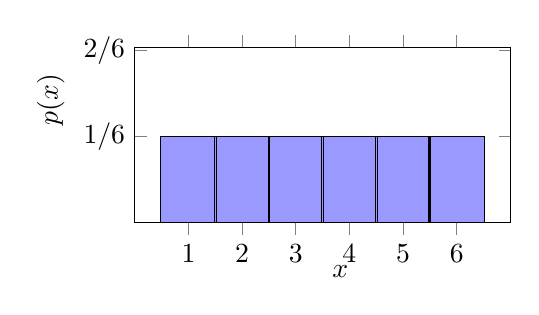
\begin{tikzpicture}
    \begin{axis}[
        ybar, % Specifies vertical bars
        ymin=0, % Ensures bars start from zero
        xtick=data, % Places x-axis ticks at data points
                     xticklabels={1,2,3,4,5,6}, % Custom x-axis labels
                    ytick       = {1/6, 2/6},
            yticklabels =  {$1/6$, $2/6$},
        enlarge x limits={0.2}, % Adjusts spacing between bars and axis limits
            y label style={anchor=south west},
            ylabel={$p(x)$},
                        xlabel = {$x$},
		x label style={anchor=west},
		 ymin = 0, ymax = .34,
        bar width=20pt, % Adjusts the width of the bars
                    width = 2.5in, height=1.5in,
       % legend style={at={(0.5,-0.15)},anchor=north,legend columns=-1} % Legend positioning
    ]
%   \addplot[fill=blue!40] coordinates {(1,0)  (2,0)  (3,0) (4,0) (5,0) (6,0) };
    \addplot[fill=blue!40] coordinates {(1,0.167)  (2,0.167)  (3,0.167) (4,0.167) (5,0.167) (6,0.167) };
    \end{axis}
\end{tikzpicture}
\task* Find $\ds P(X\leq 6)=P(X=1)+P(X=2)+P(X=3)+P(X=4)+P(X=5)+P(X=6)$\\
\blue{$\ds P(X\leq 6)=\frac{1}{6}+\frac{1}{6}+\frac{1}{6}+\frac{1}{6}+\frac{1}{6}+\frac{1}{6}=\frac{6}{6}=1$: Notation $\ds P(X\leq 6)=\sum_{k=1}^6 P(X=k) $}     \vs{.25}
}
\important{\blue{\bf Key Properties of Probability Mass Functions}}{
\enum{
\item A single probability: \blue{ $0\leq P(X=k) \leq 1$. In above example, $P(X=k)=\dfrac{1}{6}$ for all $k=1,2,3,4,5,6$} \vs{.25}
\item The sum of all probabilities:  \blue{equals 1.  In above example $\ds \sum_{k=1}^6P(X=k)=\sum_{k=1}^6 \frac{1}{6}=1$ }  \vs{.25}
}
}
%%%%%%%%%%%
%%%%%%%%%%%
%%%%%%%%%%%
\newpage
\exercise{\bf\color{Orange}P1} Let's re-consider the experiment in Exercise A (c). \\
\mpageT{.5}{.5}{We had a sample space of $$S=\{RG, RB, GR, GB,BR,BG\}$$
}{
Suppose $X$ is a discrete random variable  where $X$ is the number of blue marbles in one event. For example
\itemC{
\item  For example, $X=0$ represents the event that neither of the two drawn marbles is blue. 
\item $X=1$ represents the event that one of the marbles drawn is blue.
}
}
\vs{.2}
\tasksA{2}{
\task Find $P(X=0)$ and $P(X=1)$.
\itemI{
\item $P(X=0)=\blue{\dfrac{2}{6}=\dfrac{1}{3}}$\vs{.25}
\item $P(X=1)=\blue{\dfrac{4}{6}=\dfrac{2}{3}}$
}
\task Sketch a histogram representing this probability mass function.
\begin{center}
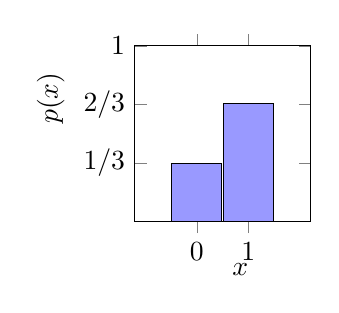
\begin{tikzpicture}
    \begin{axis}[
        ybar, % Specifies vertical bars
        bar shift=0,
        ymin=0, % Ensures bars start from zero
        xtick=data, % Places x-axis ticks at data points
                     xticklabels={0,1}, % Custom x-axis labels
                    ytick       = {1/3, 2/3,1},
            yticklabels =  {$1/3$, $2/3$,$1$},
        enlarge x limits={0.2}, % Adjusts spacing between bars and axis limits
            y label style={anchor=south west},
            ylabel={$p(x)$},
                        xlabel = {$x$},
		x label style={anchor=west},
		 ymin = 0, ymax = 1,
        bar width=18pt, % Adjusts the width of the bars
                    width = 1.5in, height=1.5in,
                    enlarge x limits={1.2}
       % legend style={at={(0.5,-0.15)},anchor=north,legend columns=-1} % Legend positioning
    ]
    %\addplot[fill=blue!40] coordinates {(1,0)  (2,0) };
    \addplot[fill=blue!40] coordinates {(1,.33)  (2,.67) };
    \end{axis}
\end{tikzpicture}
\end{center}
}



\exercise{\bf\color{Orange}P1}
\tasksA{2}{
\task     Fill in the missing probability in the table below to make it a valid probability mass function. You will want to consider the two  Key Properties of Probability Mass Functions.\\\\
{\renewcommand{\arraystretch}{1.5}
        \begin{tabular}{c|cccc}
            \hline
           $x$  & 1 & 2 & 3 & 4 \\
           \hline
           $p(x)$  & 0.1 & 0.15 &\mbox{\blue{$0.35$}}& 0.40\\
           \hline
        \end{tabular}
        }~\\
        \sol{The Key Property that we want to use is $\#2$: ``The sum of all probabilities must be $1$".
        \al{
        p(1)+p(2)+p(3)+p(4)&=1\\
        0.1+0.15+p(3)+0.4&=1\\
        0.65+p(3)&=1\\
        p(3)&=1-0.65\\
        p(3)=0.35
        }
        }
\task   Based on the probability mass function in part (a), find $P(X\ge 2)$.
\sol{
\al{
P(X\ge 2)&=P(X=2)+P(X=3)+P(X=4)\\
&=0.15+0.35+0.40\\
&=0.9=90\%
}
}
 \vs{1.7}
\task Based on the probability mass function in part (a), find $P(X \text{ is even})$.
\sol{
\al{
P(X \text{ is even })&=P(X=2)+P(X=4)\\
&=0.15+0.50\\
&=0.55
}
}
\task Sketch a histogram for this probability mass function $p(x)$.
\begin{center}
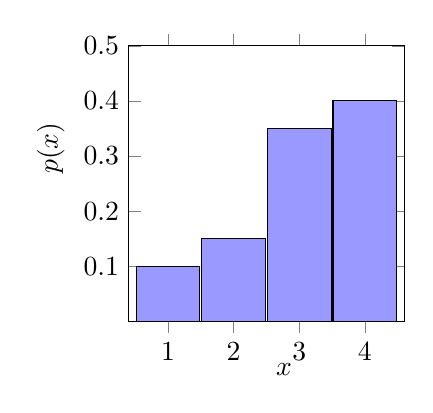
\begin{tikzpicture}
    \begin{axis}[
        ybar, % Specifies vertical bars
        bar shift=0,
        ymin=0, % Ensures bars start from zero
        xtick=data, % Places x-axis ticks at data points
                     xticklabels={1,2,3,4}, % Custom x-axis labels
                    ytick       = {0.1, 0.2, 0.3, 0.4, 0.5},
            %yticklabels =  {,,$1/3$, $2/3$,$1$},
        enlarge x limits={0.2}, % Adjusts spacing between bars and axis limits
            y label style={anchor=south west},
            ylabel={$p(x)$},
                        xlabel = {$x$},
		x label style={anchor=west},
		 ymin = 0, ymax = .5,
        bar width=23pt, % Adjusts the width of the bars
                    width = 2in, height=2in,
                    %enlarge x limits={1.2}
       % legend style={at={(0.5,-0.15)},anchor=north,legend columns=-1} % Legend positioning
    ]
 %   \addplot[fill=blue!40] coordinates {(1,0)  (2,0)  (3,0) (4,0)};
    \addplot[fill=blue!40] coordinates {(1,0.1)  (2,0.15)  (3,0.35) (4,0.4)};
    \end{axis}
\end{tikzpicture}
\end{center}
}

%%%%%%%%%%%%%
%%%%%%%%%%%%
%%%%%%%%%%%%%
\newpage



\exercise{\bf\color{Orange}P1} Two fair six-sided dice are rolled and the result of each die is recorded. Below is a table of all possible outcomes. Let $X$ be the sum of the two resulting numbers. 
\graphicsC{sum2Dice}{4}
Note that this table is one way to represent the sample space $S$ for rolling two dice and recording the outcomes.  We are assuming that  first rolling a 2 and then a 1 is distinct from first rolling a 1 and then a 2 even though both result in a sum of $3$.  
\tasksA{2}{
\task  How many different ways can two dice be rolled? 
\sol{
$6\times 6=36$
}
\task What is $P(X=4)$?  It might be helpful to think about how many total combinations of dice rolls will yield a sum of 4 relative to the total possible number of combinations that lead to our set of outcomes.
\sol{
There are $3$ ways to obtain a sum of $4$. So $\ds P(X=4)=\frac{3}{36}\approx 8.33\%$
}
\vs{1.}
\task What is $P(X\leq 4)+P(X\geq 5)$?
\sol{
This represents all possible sums so $P(X\leq 4)+P(X\geq 5)=1$!
}
\task Sketch a histogram for each of the possible sums. It might be helpful to find the probability mass functions in table below (it's ok to not convert fractions to decimals)
\begin{center}
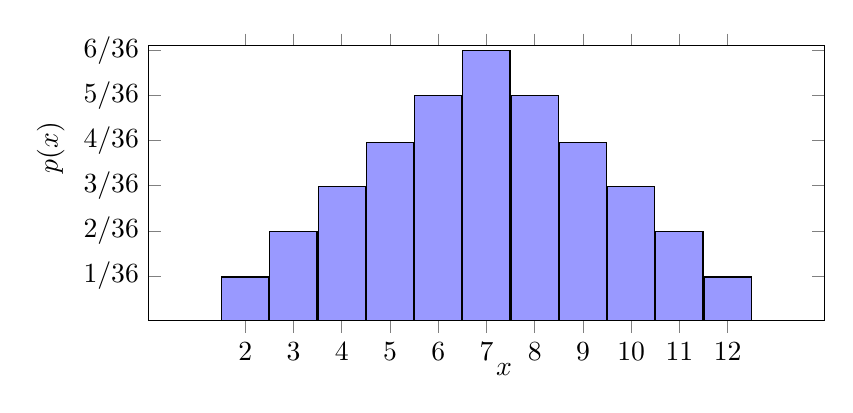
\begin{tikzpicture}
    \begin{axis}[
        ybar, % Specifies vertical bars
        bar shift=0,
        ymin=0, % Ensures bars start from zero
        xtick=data, % Places x-axis ticks at data points
                     xticklabels={2,3,4,5,6,7,8,9,10,11,12}, % Custom x-axis labels
                    ytick       = {1/36, 2/36, 3/36, 4/36, 5/36, 6/36},
            yticklabels =  {$1/36$,$2/36$,$3/36$, $4/36$,$5/36$,$6/36$},
        enlarge x limits={0.2}, % Adjusts spacing between bars and axis limits
            y label style={anchor=south west},
            ylabel={$p(x)$},
                        xlabel = {$x$},
		x label style={anchor=west},
		 ymin = 0, ymax = .17,
        bar width=17pt, % Adjusts the width of the bars
                    width = 4in, height=2in,
                    %enlarge x limits={1.2}
       % legend style={at={(0.5,-0.15)},anchor=north,legend columns=-1} % Legend positioning
    ]
% \addplot[fill=blue!40] coordinates {(1,0)  (2,0)  (3,0) (4,0) (5,0) (6,0) (7,0) (8,0) (9,0) (10,0) (11,0)};
 \addplot[fill=blue!40] coordinates {(1,0.027)  (2,0.055)  (3,0.083) (4,0.11) (5,0.139) (6,0.167) (7,0.139) (8,0.11) (9,0.083) (10,0.055) (11,0.027)};
    \end{axis}
\end{tikzpicture}
\end{center}
}
\vs{.1}
(For your convenience)\\\\
{\renewcommand{\arraystretch}{2}
        \begin{tabular}{c|ccccccccccc}
            \hline
           $x$   &2 & 3 & 4 & 5&6&7&8&9&10&11&12 \\
           \hline
           $p(x)$  & \blue{$\dfrac{1}{36}$} & \blue{$\dfrac{2}{36}$} & \blue{$\dfrac{3}{36}$} & \blue{$\dfrac{4}{36}$} & \blue{$\dfrac{5}{36}$} & \blue{$\dfrac{6}{36}$}  & \blue{$\dfrac{5}{36}$} & \blue{$\dfrac{4}{36}$}. & \blue{$\dfrac{3}{36}$} & \blue{$\dfrac{2}{36}$}. & \blue{$\dfrac{1}{36}$}\\
           \hline
        \end{tabular}
}

%%%%%
%%%%%%%%
%%%%%%
\newpage 


%\begin{enumerate}[label=(\alph*)]
%    %\item What is the size of the sample space $S$ of this experiment?
%
%    %\vfill
%
%    \item Let $X$ be the sum of the two resulting numbers. Write down the probability mass function for the random variable $X$ and sketch its histogram.
%
%    \vfill\vfill\vfill
%
%    \item Find $P(X\ge 9)$.
%
%    \vfill\vfill
%
%    \item Find $P(X\text{ is a multiple of 3})$.
%
%    \vfill\vfill
%\end{enumerate}





%%%%%%%%%
\newpage%
%%%%%%%%%

{\bf\color{blue} Extra Practice 1.} \reversemarginpar\marginnote{\fbox{\bf\color{Orange} P1}}  A standard 6-sided die has been painted so that it has 2 {\color{red}red} sides, 2 {\color{ForestGreen}green} sides, and 2 {\color{blue}blue} sides.

\begin{itemize}
    \item[(a)] In an experiment where the die is rolled and the color of the upturned face is recorded, what is the sample space $S$?

    {\Large
    \[
    S = \unlineb{4}{\{R, G,B \}}
    \]
    }
    
    \item[(b)] In an experiment where the die is rolled twice and the color of the upturned face is recorded each time, what is the sample space $S$?

    {\Large
    \[
    S = \unlineb{4}{\{RR,RG,RB, GR,GG,GB,BR,BG,BB  \}}
    \]
    }
    
\end{itemize}

{\bf\color{blue}Extra Practice 2.}\reversemarginpar\marginnote{\fbox{\bf\color{Orange} P1}} 
The World Series is the annual championship series of Major League Baseball. Currently, its format is a direct competition between two teams of up to seven games, where the first team wins four games wins the championship.

For example, if team A wins the first 3 games, team B wins the 4th game, and team A wins the 5th game, then team A wins the series. Game 6 and Game 7 will then not be played since a winner has already been determined. In this case, it took 5 games to determine the winner.

    \begin{enumerate}
    \item[(a)] Let $X$ represent the number of games it takes to determine the winner of the World Series. What are all possible values of $X$?
    \sol{
    $$S=\{ 4,5,6,7\}$$
    }
    \vfill

    \item[(b)] Suppose team A won the first 2 games and team B won the third. For each of the remaining four games, assume each team has an equal chance of winning. 

    Find $P(X\le 5)$.
\sol{
In this situation, $3$ games have been played with team A winning $2$ and team B having won $1$ game. 
\itemI{
\item Team A needs $2$ more games to win the World Series (i.e. after total of $5$ games played) 
\item Team B needs $3$ more games to win (i.e. after a total of at least $6$ games played)
}
Since no one can win after $4$ games played  $$P(X=4)=0.$$
\itemI{
\item Team $B$ cannot win the World Series in $5$ games since they need at least $6$ to win. Thus $P(\text{Team B wins in $5$ games})=0$
\item However Team A can win in $5$ games if they win the next two games.
\item Since both teams have a $50\%$ chance to win each game, \\$P(\text{Team A wins in $5$ games})=(0.5)\cdot(0.5)=0.25$
}
Thus $$P(X=5)=P(\text{Team A wins in $5$ games})+P(\text{Team B wins in $5$ games})=0.25+0=0.25$$
\al{
P(X\le 5)&=P(X=4)+P(X=5)\\
&=0+0.25\\
&=0.25
}
There is a $25\%$ chance a team will win the World Series in $5$ games or less.


 }

    \vfill

    \end{enumerate}

\end{document}

%%%%%%%%%
\newpage%
%%%%%%%%%

\begin{center}
({\it Conditioning \& Independence})
\end{center}

\begin{itemize}
    \item If $E$ and $F$ are both events, then the {\bf intersection} $E\cap F$ of both events is the event whose outcomes are in both $E$ and $F$; in other words, $E\cap F$ is the event that both $E$ and $F$ occur.
    \item If $E$ and $F$ are both events, then the event $E|F$ is the event that $E$ occurs given the condition that $F$ has already occurred. The knowledge that an event has already occurred can change how we think about possible outcomes and thus probabilities.
    \item Two events $E$ and $F$ are called {\bf independent} if knowledge that $F$ has occurred does not change the probability that $E$ occurs; that is,
    \[P(E|F)=P(E)\]
\end{itemize}

\exercise\lt{{\bf\color{Orange}P1}} A coin is flipped three times, and the upturned face is recorded after each flip. Assume each outcome - heads or tails - is equally likely for each flip.
    \begin{itemize}
    \item[(a)] What is the sample space $S$ of this experiment?

    {\Large
    \[
    S = \rule[-8pt]{5in}{0.4pt}
    \]
    }
    
    \item[(b)] Let $E_1$ be the event that the first flip lands on heads. What is $E_1$?

    {\Large
    \[
    E_1 = \rule[-8pt]{4in}{0.4pt}
    \]
    }
    
    \item[(c)] Let $E_2$ be the event that the second flip lands on heads. What is $E_2$?

    {\Large
    \[
    E_2 = \rule[-8pt]{4in}{0.4pt}
    \]
    }

    \item[(d)] What is $E_2|E_1$? Describe $E_2|E_1$ in the given context in words, as well.

    {\Large
    \[
    E_2|E_1 = \rule[-8pt]{4in}{0.4pt}
    \]
    }

    \vfill

    \item[(e)] Find the probability that $E_1$ occurs, the probability that $E_2$ occurs, and the probability that $E_2|E_1$ occurs. Are $E_1$ and $E_2$ independent? Explain.\\

    \vfill
        
    {\large
        \,\hfill
        $P(E_1)=$\rule[-8pt]{1.25in}{0.4pt}
        \hfill
        $P(E_2)=$\rule[-8pt]{1.25in}{0.4pt}
        \hfill
        $P(E_2|E_1)=$\rule[-8pt]{1.25in}{0.4pt}
        \hfill\,\\
    }
    
    \end{itemize}

%%%%%%%%%
\newpage%
%%%%%%%%%

{\bf\color{blue}Extra Practice 3.}\lt{{\bf\color{Orange}P1}} Suppose we toss two 4-sided dice - one painted {\color{red}red} and one painted {\color{blue}blue} - and record the result as an ordered pair $(\rule[-2pt]{0.2in}{0.4pt},\rule[-2pt]{0.2in}{0.4pt})$ with the first coordinate referring to the value of the {\color{red}red} die and the second coordinate referring to the value of the {\color{blue}blue} die. Assume each outcome - 1, 2, 3, or 4 - is equally likely for both dice.
    \begin{itemize}
    \item[(a)] Fill in the sample space $S$:

    {\Large 
    \begin{align*}
    S = \bigg\{ &\big( \rule[-4pt]{0.5in}{0.4pt}, \rule[-4pt]{0.5in}{0.4pt} \big), \, \big( \rule[-4pt]{0.5in}{0.4pt}, \rule[-4pt]{0.5in}{0.4pt} \big), \, \big( \rule[-4pt]{0.5in}{0.4pt}, \rule[-4pt]{0.5in}{0.4pt} \big), \, \big( \rule[-4pt]{0.5in}{0.4pt}, \rule[-4pt]{0.5in}{0.4pt} \big),\\[0.1in]
    &\big( \rule[-4pt]{0.5in}{0.4pt}, \rule[-4pt]{0.5in}{0.4pt} \big), \, \big( \rule[-4pt]{0.5in}{0.4pt}, \rule[-4pt]{0.5in}{0.4pt} \big), \, \big( \rule[-4pt]{0.5in}{0.4pt}, \rule[-4pt]{0.5in}{0.4pt} \big), \, \big( \rule[-4pt]{0.5in}{0.4pt}, \rule[-4pt]{0.5in}{0.4pt} \big),\\[0.1in]
    &\big( \rule[-4pt]{0.5in}{0.4pt}, \rule[-4pt]{0.5in}{0.4pt} \big), \, \big( \rule[-4pt]{0.5in}{0.4pt}, \rule[-4pt]{0.5in}{0.4pt} \big), \, \big( \rule[-4pt]{0.5in}{0.4pt}, \rule[-4pt]{0.5in}{0.4pt} \big), \, \big( \rule[-4pt]{0.5in}{0.4pt}, \rule[-4pt]{0.5in}{0.4pt} \big),\\[0.1in]
    &\big( \rule[-4pt]{0.5in}{0.4pt}, \rule[-4pt]{0.5in}{0.4pt} \big), \, \big( \rule[-4pt]{0.5in}{0.4pt}, \rule[-4pt]{0.5in}{0.4pt} \big), \, \big( \rule[-4pt]{0.5in}{0.4pt}, \rule[-4pt]{0.5in}{0.4pt} \big), \, \big( \rule[-4pt]{0.5in}{0.4pt}, \rule[-4pt]{0.5in}{0.4pt} \big) \bigg\}
    \end{align*}
    }

    \item[(b)] Let $E$ be the event that the sum of the displayed values is at least $7$. What is $E$? What is $P(E)$?

    {\Large
    \[
    E = \rule[-8pt]{4in}{0.4pt} \quad \& \quad P(E) = \rule[-8pt]{1in}{0.4pt}
    \]
    }

    \item[(c)] %By accident, we toss the dice so that one of the dice falls off the table onto which we tossed the dice initially, obscuring its value from our view. On the table, however, we see that the red die displays $4$.
    Let $F$ be the event that the {\color{red}red} die displays $4$. What is $F$? What is $P(F)$?

    {\Large
    \[
    F = \rule[-8pt]{4in}{0.4pt} \quad \& \quad P(F) = \rule[-8pt]{1in}{0.4pt}
    \]
    }
    \item[(d)] Describe $E|F$ in the given context in words. What is $E|F$ as a set?

    \vfill

    {\Large
    \[
    E|F = \rule[-8pt]{4in}{0.4pt}
    \]
    }
    \item[(e)] Find $P(E|F)$, and decide whether $E$ and $F$ are independent events.
    
    \vfill
    
    {\Large \hfill $P(E|F)=\rule[-8pt]{1in}{0.4pt}$}
    \end{itemize}
%%%%%%%%%%%%%%%%
\newpage
%%%%%%%%%%%%%%
{\bf\color{blue}Extra Practice 4.}\lt{{\bf\color{Orange}P1}} Many board games use strange dice. Suppose in one such game we toss one standard six-sided die and one four-sided die in a game. Assume each outcome - 1, 2, 3, 4, 5, or 6 - is equally likely for the six-sided die and each outcome 1, 2, 3, or 4 is equally likely for the four-sided die. Further, lets suppose we always roll the six-sided die first and the four-sided die second.

    \begin{itemize}
    \item[(a)] Fill in the sample space $S$:
     \begin{align*}
    S = \bigg\{
        &(\rule[-4pt]{0.3in}{0.4pt}, \rule[-4pt]{0.3in}{0.4pt}), \, (\rule[-4pt]{0.3in}{0.4pt}, \rule[-4pt]{0.3in}{0.4pt}), \, (\rule[-4pt]{0.3in}{0.4pt}, \rule[-4pt]{0.3in}{0.4pt}), \, (\rule[-4pt]{0.3in}{0.4pt}, \rule[-4pt]{0.3in}{0.4pt}), \, (\rule[-4pt]{0.3in}{0.4pt}, \rule[-4pt]{0.3in}{0.4pt}), \, (\rule[-4pt]{0.3in}{0.4pt}, \rule[-4pt]{0.3in}{0.4pt}) \\[5pt]
        &(\rule[-4pt]{0.3in}{0.4pt}, \rule[-4pt]{0.3in}{0.4pt}), \, (\rule[-4pt]{0.3in}{0.4pt}, \rule[-4pt]{0.3in}{0.4pt}), \, (\rule[-4pt]{0.3in}{0.4pt}, \rule[-4pt]{0.3in}{0.4pt}), \, (\rule[-4pt]{0.3in}{0.4pt}, \rule[-4pt]{0.3in}{0.4pt}), \, (\rule[-4pt]{0.3in}{0.4pt}, \rule[-4pt]{0.3in}{0.4pt}), \, (\rule[-4pt]{0.3in}{0.4pt}, \rule[-4pt]{0.3in}{0.4pt}) \\[5pt]
        &(\rule[-4pt]{0.3in}{0.4pt}, \rule[-4pt]{0.3in}{0.4pt}), \, (\rule[-4pt]{0.3in}{0.4pt}, \rule[-4pt]{0.3in}{0.4pt}), \, (\rule[-4pt]{0.3in}{0.4pt}, \rule[-4pt]{0.3in}{0.4pt}), \, (\rule[-4pt]{0.3in}{0.4pt}, \rule[-4pt]{0.3in}{0.4pt}), \, (\rule[-4pt]{0.3in}{0.4pt}, \rule[-4pt]{0.3in}{0.4pt}), \, (\rule[-4pt]{0.3in}{0.4pt}, \rule[-4pt]{0.3in}{0.4pt}) \\[5pt]
        &(\rule[-4pt]{0.3in}{0.4pt}, \rule[-4pt]{0.3in}{0.4pt}), \, (\rule[-4pt]{0.3in}{0.4pt}, \rule[-4pt]{0.3in}{0.4pt}), \, (\rule[-4pt]{0.3in}{0.4pt}, \rule[-4pt]{0.3in}{0.4pt}), \, (\rule[-4pt]{0.3in}{0.4pt}, \rule[-4pt]{0.3in}{0.4pt}), \, (\rule[-4pt]{0.3in}{0.4pt}, \rule[-4pt]{0.3in}{0.4pt}), \, (\rule[-4pt]{0.3in}{0.4pt}, \rule[-4pt]{0.3in}{0.4pt}) 
    \bigg\}
       \end{align*}
    

    \item[(b)] Lets suppose that you are in a position to win the game, but the sum of the numbers on the upturned faces of your next dice roll must be at least $8$. Let $E$ be the event that the sum of the displayed values on your next roll is at least $8$. What is $E$? What is $P(E)$?

    {\Large
    \[
    E = \rule[-8pt]{4in}{0.4pt} \quad \& \quad P(E) = \rule[-8pt]{1in}{0.4pt}
    \]
    }

    \item[(c)] %By accident, we toss the dice so that one of the dice falls off the table onto which we tossed the dice initially, obscuring its value from our view. On the table, however, we see that the red die displays $4$.
    Let $F$ be the event that the four-sided die displays $2$. What is $F$ as an set? What is $P(F)$?

    {\Large
    \[
    F = \rule[-8pt]{4in}{0.4pt} \quad \& \quad P(F) = \rule[-8pt]{1in}{0.4pt}
    \]
    }
    \item[(d)] %By accident, we toss the dice so that one of the dice falls off the table onto which we tossed the dice initially, obscuring its value from our view. On the table, however, we see that the red die displays $4$.
    Let $G$ be the event that the four-sided die displays $4$. What is $G$ as an set? What is $P(G)$?

    {\Large
    \[
    G = \rule[-8pt]{4in}{0.4pt} \quad \& \quad P(G) = \rule[-8pt]{1in}{0.4pt}
    \]
    }
    \item[(e)] Describe $E|F$ in the given context in words. What is $E|F$ as a set?
    \vspace{3in}

    \vfill

    {\Large
    \[
    E|F = \rule[-8pt]{4in}{0.4pt}
    \]
    }
    \item[(f)] Describe $E|G$ in the given context in words. What is $E|G$ as a set?
    \vspace{2in}

    \vfill

    {\Large
    \[
    E|G = \rule[-8pt]{4in}{0.4pt}
    \]
    }
    \item[(g)] Find $P(E|F)$, and decide whether $E$ and $F$ are independent events.

    \vfill

    {\Large \hfill $P(E|F)=\rule[-8pt]{1in}{0.4pt}$}
    \item[(h)] Find $P(E|G)$, and decide whether $E$ and $G$ are independent events.

    \vfill

    {\Large \hfill $P(E|G)=\rule[-8pt]{1in}{0.4pt}$}
    \item[(i)] Which of the two events gives you a better chance of winning, $F$ or $G$? Explain.

    \vfill

    \end{itemize}
%%%%%%%%%
\newpage%
%%%%%%%%%
\textbf{\color{blue}Extra Practice 5.}\lt{{\bf\color{Orange}P1}} Suppose we spin two spinners - one painted {\color{red}red} and one painted {\color{blue}blue} - and record the result as an ordered pair $(\rule[-2pt]{0.2in}{0.4pt},\rule[-2pt]{0.2in}{0.4pt})$ with the first coordinate referring to the color of the {\color{red}red} spinner and the second coordinate referring to the color of the {\color{blue}blue} spinner. Each spinner has three equal-sized sectors, colored {\color{ForestGreen}green}, {\color{purple}purple}, and {\color{orange}orange}. Assume each outcome -- {\color{ForestGreen}G}, {\color{purple}P}, and {\color{orange}O} -- is equally likely for both spinners.

\begin{itemize}
    \item[(a)] Fill in the sample space $S$:

    {\Large
    \begin{align*}
    S = \bigg\{ &\big( \rule[-4pt]{0.5in}{0.4pt}, \rule[-4pt]{0.5in}{0.4pt} \big), \, \big( \rule[-4pt]{0.5in}{0.4pt}, \rule[-4pt]{0.5in}{0.4pt} \big), \, \big( \rule[-4pt]{0.5in}{0.4pt}, \rule[-4pt]{0.5in}{0.4pt} \big), \\
    &\big( \rule[-4pt]{0.5in}{0.4pt}, \rule[-4pt]{0.5in}{0.4pt} \big), \, \big( \rule[-4pt]{0.5in}{0.4pt}, \rule[-4pt]{0.5in}{0.4pt} \big), \, \big( \rule[-4pt]{0.5in}{0.4pt}, \rule[-4pt]{0.5in}{0.4pt} \big), \\
    &\big( \rule[-4pt]{0.5in}{0.4pt}, \rule[-4pt]{0.5in}{0.4pt} \big), \, \big( \rule[-4pt]{0.5in}{0.4pt}, \rule[-4pt]{0.5in}{0.4pt} \big), \, \big( \rule[-4pt]{0.5in}{0.4pt}, \rule[-4pt]{0.5in}{0.4pt} \big) \bigg\}
    \end{align*}
    }

    \item[(b)] Let $E$ be the event that both spinners land on the same color. What is $E$? What is $P(E)$?

    {\Large
    \[
    E = \rule[-8pt]{4in}{0.4pt} \quad \& \quad P(E) = \rule[-8pt]{1in}{0.4pt}
    \]
    }

    \item[(c)] Let $F$ be the event that the {\color{red}red} spinner lands on {\color{purple}purple}. What is $F$? What is $P(F)$?

    {\Large
    \[
    F = \rule[-8pt]{4in}{0.4pt} \quad \& \quad P(F) = \rule[-8pt]{1in}{0.4pt}
    \]
    }

    \item[(d)] Describe $E|F$ in the given context in words. What is $E|F$ as a set?

    \vfill

    {\Large
    \[
    E|F = \rule[-8pt]{4in}{0.4pt}
    \]
    }

    \item[(e)] Find $P(E|F)$, and decide whether $E$ and $F$ are independent events.
    
    \vfill
    
    {\Large \hfill $P(E|F)=\rule[-8pt]{1in}{0.4pt}$}
\end{itemize}


 % lesson can be extended to include 2 more extra practice problems!

%%%%%%%%%
\newpage%
%%%%%%%%%

{\bf\color{blue}Extra Practice 3.}\lt{{\bf\color{Orange}P1}} An opaque bag contains 2 {\color{red}red} marbles, 1 {\color{ForestGreen}green} marble, and 3 {\color{blue}blue} marbles. Two marbles are drawn one at a time, and the color is recorded each time.

    \begin{itemize}
    \item[(a)] What is the sample space of this experiment?\\

    {\Large
    \[
    S = \rule[-8pt]{4in}{0.4pt}
    \]
    }
        
    \item[(b)] Some events are given below. Please respond to the prompts that follow them.

        \begin{itemize}
        \item $E_{1R}$ is the event that the first marble is {\color{red}red}.
        \item $E_{2R}$ is the event that the second marble is {\color{red}red}.
        \item $E_{1G}$ is the event that the first marble is {\color{ForestGreen}green}.
        \item $E_{2G}$ is the event that the second marble is {\color{ForestGreen}green}.
        \item $E_{1B}$ is the event that the first marble is {\color{blue}blue}.
        \item $E_{2B}$ is the event that the second marble is {\color{blue}blue}.
        \end{itemize}

    Find $P(E_{2R}|E_{1R})$, $P(E_{2G}|E_{1G})$, $P(E_{2B}|E_{1B})$ if the marbles are drawn {\bf with replacement}.

    \vfill

    Find $P(E_{2R}|E_{1R})$, $P(E_{2G}|E_{1G})$, $P(E_{2B}|E_{1B})$ if the marbles are drawn {\bf without replacement}.

    \vfill
    
    \end{itemize}

%%%%%%%%%
\newpage%
%%%%%%%%%

{\bf\color{blue}Extra Practice 4.} In an experiment, a coin is flipped continually until a heads appears, at which point the experiment concludes.
    \begin{itemize}
    \item[(a)] What is the sample space of this experiment? Use $H$ to represent heads and $T$ to represent tails.

    {\Large
    \[
    S = \rule[-8pt]{4in}{0.4pt}
    \]
    }
    
    \item[(b)] Let $E_n$ denote the event that $n$ flips are necessary to complete the experiment. What points of the sample space are contained in $E_1$? in $E_2$? in $E_3$?\\

    {\large
        \,\hfill
        $E_1=$\rule[-8pt]{1.5in}{0.4pt}
        \hfill
        $E_2=$\rule[-8pt]{1.5in}{0.4pt}
        \hfill
        $E_3=$\rule[-8pt]{1.5in}{0.4pt}
        \hfill\,\\
    }

    \item[(c)] Find the following probabilities:\\

    {\large
        \,\hfill
        $P(E_1)=$\rule[-8pt]{1in}{0.4pt}
        \hfill
        $P(E_2|\{T\})=$\rule[-8pt]{1in}{0.4pt}
        \hfill
        $P(E_3|\{TT\})=$\rule[-8pt]{1in}{0.4pt}
        \hfill\,\\
        }

    \vfill

    {\large
        \,\hfill
        $P(E_2|E_1)=$\rule[-8pt]{1in}{0.4pt}
        \hfill
        $P(E_3|E_2)=$\rule[-8pt]{1in}{0.4pt}
        \hfill
        $P(E_3|E_1)=$\rule[-8pt]{1in}{0.4pt}
        \hfill\,\\
        }

    \vfill
        
    \end{itemize}
    

%%%%%%%%%%%%%%%%%%%%%%%%%%%%%%%%%%%%%%%%%%%%%%%%%%%%%%
%%%%%%%%%%%%%%%%%%%%%%%%%%%%%%%%%%%%%%%%%%%%%%%%%%%%%%
%%%%%%%%%%%%%%%%%%%%%%%%%%%%%%%%%%%%%%%%%%%%%%%%%%%%%%
%%%%%%%%%%%%%%%%%%%%%%%%%%%%%%%%%%%%%%%%%%%%%%%%%%%%%%
%% Deleted Section on Conditioning and Independence %%
%%%%%%%%%%%%%%%%%%%%%%%%%%%%%%%%%%%%%%%%%%%%%%%%%%%%%%
%%%%%%%%%%%%%%%%%%%%%%%%%%%%%%%%%%%%%%%%%%%%%%%%%%%%%%
%%%%%%%%%%%%%%%%%%%%%%%%%%%%%%%%%%%%%%%%%%%%%%%%%%%%%%
%%%%%%%%%%%%%%%%%%%%%%%%%%%%%%%%%%%%%%%%%%%%%%%%%%%%%%



